\documentclass[11pt]{ltjsarticle}

\usepackage{amsmath}
\usepackage{amssymb}
\usepackage{amsthm}
\usepackage{bm}
\usepackage[margin=25mm]{geometry}
\usepackage{hyperref}
\usepackage{graphicx}

\newcommand{\I}{I}
\newcommand{\J}{\mathbf{J}}
\newcommand{\PhiI}{\Phi}
\newcommand{\dd}{\mathrm{d}}

\newtheorem{definition}{定義}
\newtheorem{axiom}{公理}
\newtheorem{proposition}{命題}
\newtheorem{remark}{注意}

\title{Bio-IFGT: 情報流アトラクタ動力学としての生物学的形態形成}
\author{
Yuhki Endo\\
Independent Researcher
}
\date{\today}

\begin{document}

\maketitle

\begin{abstract}
本論文では、生物系を情報密度 \(\I\)、情報流 \(\J\)、および誘導ポテンシャル \(\PhiI\) によって記述する、最小かつ統一的な枠組みを提示する。この枠組みでは、DNA は完成形を符号化するものではなく、系のダイナミクスを制約するパラメータ集合 \(\theta\) として扱われる。

この立場により、発生は安定配置への収束として、形態はアトラクタ構造として、生命は動的に維持される非平衡状態として解釈される。生命誕生確率も、特定の分子構造への命中確率ではなく、状態空間における安定領域へ到達する確率として再定式化される。

知性は、生命の単なる延長ではなく、生命アトラクタの上に成立する第二のアトラクタとして位置づけられる。本論文は新しい生物学的機構を提案するものではない。最小限の動的量を用いて、生物現象に対する統一的な構造記述を与えることを目的とする。
\end{abstract}

\setcounter{tocdepth}{1}
\tableofcontents
\clearpage

\section{Introduction}

生物学における多くの現象は、発生、形態形成、分化、進化として観測される。これらはしばしば、設計、プログラム、遺伝的指令といった言葉で説明される。しかし、そのような表現と実際の物理的・化学的過程との対応は必ずしも明確ではない。

DNA 配列は分子生成や反応経路を制約するが、完成された構造、目的、意図を直接に指定するものではない。同一の DNA を持つ細胞が異なる状態へ分化しうることは、この点を示している。したがって本論文では、DNA を系のダイナミクスを制約するパラメータ集合 \(\theta\) として扱う。

本論文では、生物系を状態変化と持続構造の過程として記述する。用いる量は、情報密度 \(\I\)、情報流 \(\J\)、誘導ポテンシャル \(\PhiI\) である。これらは、発生と形態形成を共通に記述するための量である。

この枠組みの特徴は、設計や目的を説明の出発点としない点にある。形態や機能は、状態変化が安定構造へ収束した結果として現れる。

本論文の目的は、既存の現象を一貫した形式で記述することである。そのために、最小限の変数、連続方程式、安定構造としての解釈を組み合わせる。

Section 2 では直観的な見取り図を示す。Section 3 では形式的な対応関係を定義する。Section 4 では基本方程式を導入する。Section 5 以降では、生物学的現象への適用とシミュレーション例を扱う。

本論文は、Information-Field-Geometry-Theory（IFGT）に基づいている。IFGT は、系が閉包へ向かう運動と、準閉包構造の持続を定式化する。IFGT において、閉包度 \(C\) は、系が安定配置へどの程度進行したかを特徴づける。ただし、生物系で用いる \(\I\) は、IFGT 本体の \(I=f(1-C)\) と直接同一視される量ではない。ここでの \(\I\) は、生物学的観測窓において粗視化された制約密度場であり、局所的な構造制約、分化、保持された偏りを表す。この関係は変数の同一性ではなく、記述レイヤー間の対応である。生命系の持続的な非平衡構造は、IFGT の語彙では準閉包に対応する。すなわち、完全閉包境界の手前側に留まり、残差的な差異が更新に利用可能であることによって持続するレジームである。

\section{Intuitive Picture}

本節では、本論文で用いる枠組みを直観的に示す。目的は厳密な定義ではなく、どのような対象をどのように見ているかを共有することである。

\subsection{状態と変化}

生物系は固定された構造ではなく、状態が変化し続ける過程として捉えられる。分子は生成され、分解され、移動し、細胞状態は時間とともに変化する。

重要なのは、変化が止まらないにもかかわらず、全体としての構造が保たれる点である。生物学的安定性は、静止ではなく、更新の中で維持される組織化である。

\subsection{偏りと流れ}

状態変化は一様ではない。ある場所では特定の分子が多く生成され、別の場所では抑制される。このような非対称性は、状態変化に方向性を与える。本論文では、この方向性を流れと呼ぶ。

流れは、生成、拡散、移動、相互作用の総合として生じる。それは別個の実体ではなく、状態更新の正味の方向と速度である。

\subsection{安定領域}

流れが存在するとき、すべての状態が同じように振る舞うわけではない。維持されやすい状態もあれば、崩れやすい状態もある。その結果、系が繰り返し戻る領域が現れる。

このような領域は動力学的な意味で安定であり、近傍のずれを吸収し、認識可能な構造を維持する。

\subsection{形の出現}

発生や形態形成は、あらかじめ指定された形の実現ではなく、継続的な状態変化を通じて安定配置が現れる過程として解釈される。細胞分布や器官配置は、このような安定配置として観測される。

\subsection{設計仮定を使わない記述}

この見方では、目的、設計、指令を原始概念として用いない。必要なのは、状態変化、非対称性、流れ、安定配置である。

\subsection{まとめ}

生物系は、状態変化、流れ、安定構造の組み合わせとして理解できる。本論文では、この直観を情報密度 \(\I\)、情報流 \(\J\)、誘導ポテンシャル \(\PhiI\) によって定式化する。

\section{Formal Mapping}

本節では、直観的な記述を形式的な量へ対応づける。目的は、直観と数式の対応を明確にすることであり、特定の生物系の完全な導出を与えることではない。

\subsection{状態の記述}

生物系は、空間と時間に依存する状態として表される。位置 \(\mathbf{r}\in\mathbb{R}^3\)、時間 \(t\in\mathbb{R}\) に対し、すべての微視的詳細ではなく、粗視化された場を扱う。

\subsection{情報密度}

局所状態に含まれる構造や制約の偏りを、情報密度
\begin{equation}
  \I(\mathbf{r},t)
\end{equation}
として表す。ここで情報とは意味内容ではない。局所的な構造、制約、分化、相互依存の程度を表す量である。

\subsection{情報流}

状態更新の方向と速度を、情報流
\begin{equation}
  \J(\mathbf{r},t)
\end{equation}
として表す。\(\J\) は反応、拡散、移動、相互作用からの寄与をまとめたものであり、粗視化された状態がどのように更新されるかを表す。

\subsection{誘導ポテンシャル}

情報密度に空間的偏りがあるとき、状態変化には非対称性が生じる。この非対称性を誘導ポテンシャル
\begin{equation}
  \PhiI = \PhiI[\I]
\end{equation}
で表す。これは、\(\I\) の分布によって誘導される有効ポテンシャルである。対応する勾配駆動のバイアスは
\begin{equation}
  \mathbf{F}=-\nabla \PhiI
\end{equation}
と書かれる。

\subsection{流れとの関係}

情報流は拡散成分とポテンシャルにより誘導される成分の和として
\begin{equation}
  \J = -D\nabla \I + \mu \mathbf{F}
\end{equation}
と書ける。ここで \(D\) は拡散係数、\(\mu\) は応答係数である。

\subsection{時間の扱い}

運動方程式は外部時間 \(t\) によって記述する。一方で、内部の状態更新の進行量を表す内部時間 \(\tau\) を
\begin{equation}
  \frac{\dd \tau}{\dd t}=\rho(\I,\J)
\end{equation}
として導入できる。本論文では、運動方程式は \(t\) で記述し、\(\tau\) は解釈に用いる。

\subsection{まとめ}

対応関係は、偏りや制約が \(\I\)、状態更新が \(\J\)、更新の非対称性が \(\PhiI\) である。この対応により、直観的な見取り図は連続場の記述へ変換される。

\section{Core Equations}

本節では、本論文で用いる最小方程式系を導入する。これらの式は特定の生物系に依存せず、状態変化、流れ、安定構造を共通に扱うための一般形式である。

\subsection{基本変数}

基本となる場は、情報密度
\begin{equation}
  \I(\mathbf{r},t)
\end{equation}
と情報流
\begin{equation}
  \J(\mathbf{r},t)
\end{equation}
である。\(\I\) は局所的な構造や制約の密度を表し、\(\J\) は状態変化の方向と速度を表す。

\subsection{連続方程式}

情報密度は次の連続方程式に従う。
\begin{equation}
  \frac{\partial \I}{\partial t}+\nabla\cdot\J=\sigma .
  \label{eq:ja-continuity}
\end{equation}
ここで \(\sigma(\mathbf{r},t)\) は局所的な生成率である。

\subsection{情報流の構造}

情報流は
\begin{equation}
  \J=-D\nabla \I+\mu\mathbf{F}
  \label{eq:ja-flow}
\end{equation}
と書く。ここで \(D\) は拡散係数、\(\mu\) は応答係数、\(\mathbf{F}\) は誘導された方向場である。

\subsection{ポテンシャル}

方向場は誘導ポテンシャルにより
\begin{equation}
  \mathbf{F}=-\nabla\PhiI
  \label{eq:ja-force}
\end{equation}
と定まる。ポテンシャルは情報密度の汎関数として
\begin{equation}
  \PhiI=\PhiI[\I]
  \label{eq:ja-potential}
\end{equation}
と書く。 \(\PhiI\) の具体的な形は系に依存し、本論文では指定しない。したがって、情報密度の偏りが状態変化に勾配駆動のバイアスを与える。符号規約は \(\PhiI[\I]\) を具体的に指定した後に定まる。例えば \(\PhiI\sim-\I\) と置けば、誘導成分 \(-\nabla\PhiI\) は制約密度が増大する方向を向く。別の生物学的観測量では、逆の符号規約や追加の応答項が必要になる場合がある。

\subsection{動力学的ループ}

式 \eqref{eq:ja-continuity}--\eqref{eq:ja-potential} はループを形成する。\(\I\) の分布が \(\PhiI\) を誘導し、\(\PhiI\) が \(\J\) を形づくり、\(\J\) が \(\I\) を再配置する。このループは必ずしも静的平衡で終わらず、継続的更新の下で維持される非平衡構造を生みうる。

\subsection{時間の二層構造}

方程式は外部時間 \(t\) を用いて書く。内部時間 \(\tau\) は
\begin{equation}
  \frac{\dd \tau}{\dd t}=\rho(\I,\J)
\end{equation}
として導入され、系内部の進行を解釈するために用いられる。

\subsection{安定構造}

この動力学のもとで、状態がある領域に留まり、摂動後にも戻る傾向を持つとき、その領域はアトラクタとして解釈される。

\subsection{まとめ}

最小方程式系は
\begin{align}
  \frac{\partial \I}{\partial t}+\nabla\cdot\J&=\sigma,\\
  \J&=-D\nabla\I+\mu\mathbf{F},\\
  \mathbf{F}&=-\nabla\PhiI,\\
  \PhiI&=\PhiI[\I]
\end{align}
である。この系により、状態変化、流れの形成、安定構造の出現を共通形式で記述する。

\section{Gene \texorpdfstring{\(\times\)}{x} Information Flow}

本節では、DNA と遺伝子関連過程を情報密度と情報流によって記述する。目的は、発生、形態、細胞運命の成立を、意味や設計の実行ではなく、状態変化の連鎖として記述することである。

\subsection{DNAの位置づけ}

DNA 配列 \(s\) は
\begin{equation}
  s\in\{A,T,G,C\}^{N}
\end{equation}
と書ける。本形式では、配列自体に意味や目的は仮定しない。DNA は分子生成の可能性、反応の起こりやすさ、閾値条件を制約する。

したがって DNA は
\begin{equation}
  \theta=\theta(s)
\end{equation}
として表されるパラメータ集合であり、完成した形態の直接指定ではない。

\subsection{遺伝子イベント}

転写、翻訳、結合、修飾は、情報密度を局所的に変化させる操作として
\begin{equation}
  \I(\mathbf{r},t)\mapsto \I(\mathbf{r},t)+\Delta\I
\end{equation}
と表せる。個々のイベントは離散的だが、その総和は連続的な情報流 \(\J(\mathbf{r},t)\) として表される。

\subsection{連続方程式との接続}

\begin{equation}
  \frac{\partial \I}{\partial t}+\nabla\cdot\J=\sigma
\end{equation}
において、\(\sigma\) は遺伝子関連イベントに起因する情報生成率を表す。\(\J\) はそれらの効果が空間と時間を通じて蓄積した流れである。

\subsection{偏りと誘導ポテンシャル}

情報密度に偏りが生じると
\begin{equation}
  \PhiI=\PhiI[\I]
\end{equation}
が誘導され、状態変化は
\begin{equation}
  \mathbf{F}=-\nabla\PhiI
\end{equation}
に従ってバイアスを受ける。これは新しい根本力ではなく、安定状態が維持されやすく、近傍状態をその basin に引き込むという動力学的性質の記述である。

\subsection{if/then 条件としての閾値}

DNA による条件的効果は、連続場における閾値条件として表される。応答関数 \(F_k\) に対して
\begin{equation}
  F_k(\I,\J,\mathbf{r},t;\theta)>\theta_k
\end{equation}
となるとき、反応が切り替わる。ここで \(\theta_k\) は DNA に由来するパラメータ集合 \(\theta\) によって与えられる。

\subsection{形態の解釈}

DNA はパラメータを与え、情報密度と情報流が形成され、\(\I\) の偏りが \(\PhiI\) を誘導し、流れが成形され、閾値が状態を分岐させる。その結果として安定配置がアトラクタとして現れる。細胞運命や形態は、そのような安定配置として観測される。

\subsection{スケール不変性}

同じ形式は、分子、細胞、組織の各スケールに用いることができる。粗視化のレベルは変わるが、\(\I\)、\(\J\)、\(\PhiI\)、閾値、安定解の役割は保たれる。

\subsection{まとめ}

DNA は条件を設定するパラメータ集合として扱われる。生物学的構造は、情報密度と情報流によって形成される安定解として現れる。この見方は、次節で扱う発生と形態形成の基盤となる。

\subsection{パラメータ集合の起源}

この記述レイヤーでは、パラメータ集合 \(\theta\) は原始的なものとして扱われない。IFGT の語彙では、\(\theta\) は差異の先行するダイナミクスを通じて安定化した準閉包構造として読むことができる。すなわち、ある閉包パターンが他のパターンよりも持続した結果として保持された配置である。したがって DNA 配列は、持続的な非平衡ダイナミクスを支えたために残った、歴史的に安定化した制約パターンとして解釈される。ただしこれは、具体的な生物における \(\theta\) の起源を導出するものではない。\(\theta\) を枠組みの外部にある説明対象として置く必要がない、ということを述べるにとどまる。

\section{Development and Morphogenesis}

本節では、前節までの枠組みを発生と形態形成へ適用する。発生は設計の実行ではなく、状態変化が安定構造へ収束する過程として解釈される。

\subsection{初期状態と非対称性}

受精卵は、状態空間の中で広い可能性を持つ初期状態にある。この段階では、情報密度はおおむね均一であり、巨視的構造はまだ固定されていない。しかし、初期条件や環境ゆらぎによる小さな非対称性が存在し、それが後の構造形成の種となりうる。

\subsection{モルフォゲンとしての情報密度}

発生過程では、モルフォゲンが空間的な濃度分布を形成する。本枠組みでは、それを
\begin{equation}
  \I(\mathbf{r},t)
\end{equation}
として扱う。局所生成は \(\I\) の勾配を生み、拡散と分解がその分布を形づくる。

\subsection{ダイナミクス}

粗視化された標準形として
\begin{equation}
  \frac{\partial \I}{\partial t}
  =D\nabla^2\I-\lambda\I+\sigma(\mathbf{r},t;\theta)
\end{equation}
を用いる。ここで \(D\) は拡散係数、\(\lambda\) は減衰率、\(\sigma\) はパラメータ集合 \(\theta\) に制約される局所生成項である。

\subsection{誘導ポテンシャルと勾配}

\(\I\) の分布は
\begin{equation}
  \PhiI=\PhiI[\I]
\end{equation}
を誘導し、状態変化は
\begin{equation}
  \mathbf{F}=-\nabla\PhiI
\end{equation}
によりバイアスされる。この偏りが構造形成に方向性を与える。

\subsection{閾値による分化}

細胞運命は、\(\I\) に対する閾値によって分岐しうる。
\begin{align}
  \I(\mathbf{r})<\theta_1 &\Rightarrow \text{state A},\\
  \theta_1\leq\I(\mathbf{r})<\theta_2 &\Rightarrow \text{state B},\\
  \I(\mathbf{r})\geq\theta_2 &\Rightarrow \text{state C}.
\end{align}
\(\I\) は連続量であり、観測される結果は離散的に現れる。分化は、連続的状態変化への閾値応答として理解される。

\subsection{アトラクタとしての形態}

ダイナミクスと閾値構造の組み合わせにより、分布が安定化し、分化パターンが固定される。この安定状態が、発生における形態として観測される。

\subsection{頑健性}

発生の再現性と頑健性は、複数の初期条件が同一の安定配置へ収束しうるというアトラクタ構造から説明できる。局所的なゆらぎは、ダイナミクスによって吸収される。

\section{Life as Attractor}

本節では、生命を完成された物体ではなく、状態空間における持続的な安定構造として定式化する。この視点により、維持、発生、分化、再生を同一の動力学的枠組みで扱うことができる。

\subsection{状態空間による記述}

生物系は状態ベクトル
\begin{equation}
  x(t)=(x_1(t),x_2(t),\ldots,x_n(t))
\end{equation}
で表される。成分には、分子濃度、発現レベル、反応速度、局所環境などが含まれる。時間発展は
\begin{equation}
  \frac{\dd x}{\dd t}=F(x;\theta)
\end{equation}
で与えられる。ここで \(\theta\) は DNA に由来する制約を表すパラメータ集合である。

\subsection{内部時間}

外部時間 \(t\) に加えて、内部の状態更新の進行を表す内部時間 \(\tau\) を
\begin{equation}
  \frac{\dd\tau}{\dd t}=\rho(x)
\end{equation}
として導入する。\(\tau\) は状態変化や情報更新の蓄積を表し、一般には \(t\) と一致しない。

\subsection{生命の定義}

生命は単一の状態ではない。ある領域に留まりながら変化し続ける運動である。すなわち、静止せず、無制限に発散せず、一定の範囲に拘束される。このとき \(\tau\) は継続的に進行する。

\subsection{生命アトラクタ}

状態空間 \(\Omega\) の中に
\begin{equation}
  \Omega_{\mathrm{life}}\subset\Omega
\end{equation}
があり、系がそこに入ると摂動後にも戻る傾向を持つとき、それを生命アトラクタと呼ぶ。この領域は外部から与えられるものではなく、相互作用を通じて形成される。

\subsection{非平衡持続構造}

生命アトラクタは平衡状態ではない。物質は流入し、分子は入れ替わり、エネルギーは消費される。それにもかかわらず組織化は維持される。生命は、非平衡状態における持続構造である。

\subsection{分化とサブアトラクタ}

生命アトラクタ内部には、より具体的な安定領域が存在しうる。細胞分化は、\(\Omega_{\mathrm{life}}\) 内のサブアトラクタへの遷移として解釈できる。

\section{Probability Revision}

本節では、生命誕生確率の定式化を再検討する。目的は数値を与えることではなく、何を確率として数えるのかを明確にすることである。

\subsection{従来の定式化}

生命誕生はしばしば、特定の分子構造が偶然に成立する確率として扱われる。この見方では、多数の条件が同時に満たされる必要があり、全体確率は小さくなる。この見方は、生命を特定の完成配置とみなす限り一貫している。

\subsection{問題の所在}

本論文では、生命を固定構造ではなく、状態空間における持続的な安定運動とみなす。このとき生命は一点ではなく、有限の広がりを持つ領域に対応する。生命誕生は、特定構造への命中ではなく、その領域へ到達し、そこに留まることとして捉え直される。

\subsection{領域としての確率}

生命アトラクタの領域を
\begin{equation}
  \Omega_{\mathrm{life}}\subset\Omega
\end{equation}
とする。生命誕生確率は、\(\Omega_{\mathrm{life}}\) に到達する確率である。これは一点への命中確率ではなく、領域への侵入確率である。

\subsection{試行の構造}

分子反応や物質循環は、条件が続く限り繰り返される。持続しない状態は消え、持続する状態だけが残る。この意味で、生命はあらかじめ選ばれるのではなく、持続しうる状態として現れる。

\subsection{次元の縮約}

点を目標とする見方では、多数の自由度を同時に指定する必要がある。一方、本枠組みでは、生命成立条件は安定領域への到達を特徴づける少数の有効変数で表される。したがって、確率問題の構造そのものが変わる。

\subsection{解釈}

これは確率値の再評価ではなく、数えられる対象の構造的再定義である。生命は奇跡的な命中でも、自動的必然でもない。維持条件が存在するときに現れうる状態である。

IFGT の語彙では、この再定式化は明確な解釈を持つ。生命は、準閉包レジームへの到達とその内部での持続に対応する。準閉包レジームとは、閉包へ向かう駆動が維持されながら、完全閉包境界が通常の状態としては到達されない動力学的領域である。したがって生命の確率は、固定された分子配置を組み立てる確率ではなく、そのようなレジームへ到達し維持される確率として理解する方が適切である。生命が極端に低確率に見えることは、少なくとも部分的には、何を標的として同定したかに依存している可能性がある。

\section{Intelligence as a Second Attractor}

本節では、知性を生命の単なる延長ではなく、生命アトラクタの上に成立する第二の安定構造として扱う。

\subsection{知性の位置づけ}

生命はすでにアトラクタ構造として成立している。多くの生命系は、そのアトラクタ内で長期間持続するが、自動的に知性へ至るわけではない。したがって知性は生命アトラクタの単なる強化ではない。

\subsection{第二のアトラクタ}

知性は、情報が流れるだけでなく、保持され、参照され、再利用される構造として現れる。過去状態が現在に影響し、現在状態が未来の軌道を調整する。このような再帰的ループは、生命だけに必要な条件とは異なる条件のもとで安定化する。

\subsection{構造的独立性}

形式的には
\begin{equation}
  \Omega_{\mathrm{intel}}\subset\Omega_{\mathrm{life}}
\end{equation}
と書けるが、\(\Omega_{\mathrm{intel}}\) の内部構造は追加の制約によって決まる。状態履歴の持続的参照、時間的情報蓄積、複数要素間の情報共有などが必要となる。

\subsection{確率構造}

知性の成立は、生命成立とは異なる条件の成立として扱われる。概略的な因子分解として
\begin{equation}
  P_{\mathrm{intel}}\approx P_{\mathrm{life}}P_{\mathrm{second}\mid\mathrm{life}}
\end{equation}
と書ける。これは数値評価ではなく、二段階構造を示すための表現である。

\subsection{内部時間との関係}

生命は \(\tau\) が持続的に進行する構造である。一方、知性は \(\tau\) の履歴が参照され再利用される構造として特徴づけられる。この意味で、知性は単なる流れではなく、再帰的情報流である。

\section{Relation to Note}

本節では、本論文と対応する note 形式の本文との関係を整理する。目的は理論の要約ではなく、同じ構造が異なる記述レイヤーでどのように現れるかを明確にすることである。

本論文は L3 の形式層であり、note 本文は L1 の直観層である。両者は同じ対象を扱うが、目的が異なる。本論文は定義、方程式、関係を固定し、note 本文は比喩や読みやすい表現によって直観的理解を助ける。重要なのは、文言の一致ではなく構造の対応である。

本論文の \(\I\) は note では「かたまり」「偏り」「構造がある場所」として、\(\J\) は「流れ」「くり返し」「通りやすさ」として、\(\PhiI\) は「引き戻される感じ」「落ち着く場所」として現れる。アトラクタは「同じところに戻る」「かたちが保たれる」という表現に対応する。

発生と形態形成は、note では「くり返すと変わる」「流れができる」「かたちになる」といった形で表現される。生命は「物ではなく状態である」として説明される。確率の再定義は「奇跡ではない」という表現に対応する。

\section{Minimal Developmental Simulation (Bio-IFGT Toy Model)}

\subsection{目的}

本節では、Bio-IFGT の最小玩具モデルを導入する。目的は、局所源、拡散、減衰、閾値、応答率からなる小さな DNA 的パラメータ集合が、幾何学を明示的に指定しなくても安定した生物様構造を生みうることを示すことである。

\subsection{モデル設定}

胚様の二次元領域を考える。系は離散時間で発展し、主要な場として、モルフォゲン場 \(M(x,y,t)\)、情報密度 \(\I(x,y,t)\)、神経コミットメント \(N(x,y,t)\)、眼様コミットメント \(E(x,y,t)\) を持つ。また補助的に境界安定化場 \(B(x,y,t)\) を導入する。

\subsection{ダイナミクス}

モルフォゲン場は
\begin{equation}
  \frac{\partial M}{\partial t}=D_M\nabla^2M-\lambda_M M+\sigma_M(x,y)
\end{equation}
に従う。情報密度は
\begin{equation}
  \frac{\partial \I}{\partial t}=D_I\nabla^2\I-\lambda_I\I+\alpha M
\end{equation}
で更新される。神経コミットメントは
\begin{equation}
  N_{t+1}=N_t+\eta_N S(\I-\theta_N)(1-N_t)
\end{equation}
で与えられる。

境界場は情報密度の勾配から
\begin{equation}
  G=|\nabla\I|
\end{equation}
として導かれる。境界場は、空間変化が局所的に最大化される領域を表す。その更新は
\begin{equation}
  B_{t+1}=B_t+\eta_B S(G-\theta_B)(1-B_t)
\end{equation}
である。

眼様コミットメントは、神経コミットメント、境界安定化、位置窓が同時に有効な場所で
\begin{equation}
  E_{t+1}=E_t+\eta_E S(N-\theta_{EN})S(B-\theta_{EB})A(x,y)(1-E_t)
\end{equation}
として更新される。ここで
\begin{equation}
  S(z)=\frac{1}{1+e^{-kz}}
\end{equation}
である。

\subsection{解釈}

このモデルは神経構造や眼様構造の幾何学を明示的に符号化しない。局所源、拡散・減衰パラメータ、閾値条件、応答率だけを指定する。その結果、滑らかなモルフォゲン勾配、情報密度地形、神経板様領域、境界構造、眼様局在構造が階層的に現れる。

\subsection{主要な観察}

生成は
\begin{equation}
  M\rightarrow \I\rightarrow N\rightarrow B\rightarrow E
\end{equation}
という逐次的制約として進む。各段階は、スカラー場、勾配構造、閾値による離散化、複合条件による局在化を導入する。

\subsection{概念的含意}

このシミュレーションは、生物様構造が完成形として符号化されていなくても、制約された情報地形の中の安定解として現れうることを示す。DNA 的パラメータは、可能な状態の幾何を形づくる条件として働く。

\subsection{Bio-IFGTとの関係}

Bio-IFGT の枠組みでは、\(\I\) は情報密度、\(\PhiI\sim-\I\) は有効ポテンシャル地形、\(\J\sim-\nabla\PhiI\) は安定領域へ向かう流れに対応する。観測される構造は、この場のアトラクタ様配置に対応する。

生成経路 \(M\rightarrow \I\rightarrow N\rightarrow B\rightarrow E\) の各段階は、準閉包の逐次的な局在化として解釈できる。モルフォゲン場は大域的な情報勾配を形成し、それが \(\I\) の局所的蓄積を駆動する。\(\I\) は閾値を超えることで場の部分領域を安定化する。眼様コミットメント \(E\) は、神経板様領域 \(N\) に支えられつつ、それとは区別される二次的な準閉包を表す。この階層構造は、生命アトラクタ内のサブアトラクタとして分化を捉える解釈を反映している。

\subsection{限界}

このモデルは意図的に最小化された玩具モデルであり、生物学的詳細の再現を目的としない。制約されたダイナミクスのもとで構造が立ち上がるという構造原理を示すためのものである。

\section{Simulation Results and Visualization}

本節では、前節で導入した最小発生モデルに対する数値シミュレーション結果を報告する。目的は、玩具モデルの中で構造がどのように時間発展として現れるかを確認することであり、特定の生物過程の再現ではない。

\subsection{初期状態}

初期状態では、場はほぼ一様であり、組織化された構造は存在しない。モルフォゲン場 \(M\) は局所的な生成源のみを持ち、情報密度 \(\I\) は低く、小さな摂動以外に意味のある空間偏りを持たない。神経コミットメント \(N\) と眼様コミットメント \(E\) は未分化である。この状態では、完成した形に対応する情報は場のどこにも存在しない。

\subsection{時間発展}

時間発展の中で、まずモルフォゲンが拡散し滑らかな勾配を形成する。次に情報密度 \(\I\) が蓄積して空間的偏りが強まる。閾値条件により中央に神経板様領域 \(N\) が現れ、\(|\nabla\I|\) によって境界場 \(B\) が定義される。最後に、神経コミットメント、境界安定化、位置窓が重なる場所に眼様コミットメント \(E\) が局所的に現れる。

\subsection{最終状態}

最終状態では、中央に安定した神経板様領域が形成される。眼様構造は神経場の境界付近に局在して現れる。一方、中央部では関連する境界条件が弱いため、眼様場は形成されにくい。したがって、このダイナミクスは、構造が現れる場所だけでなく、現れない場所も同時に決めている。

\subsection{図の説明}

各図は、前節で述べた階層的生成の一段階に対応する。

\begin{figure}[htbp]
  \centering
  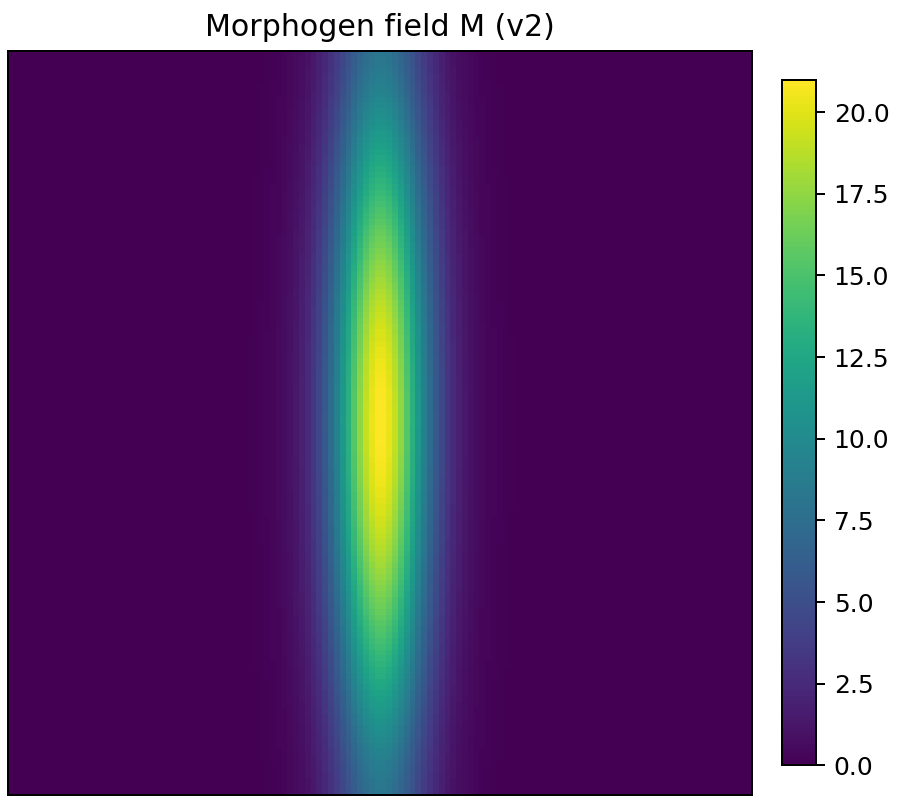
\includegraphics[width=0.70\linewidth]{simulations/minimal_neural_field/outputs/morphogen_final_v2.png}
  \caption{最終モルフォゲン場 \(M\)。中央生成源の周囲に滑らかな場が形成される。}
\end{figure}

\begin{figure}[htbp]
  \centering
  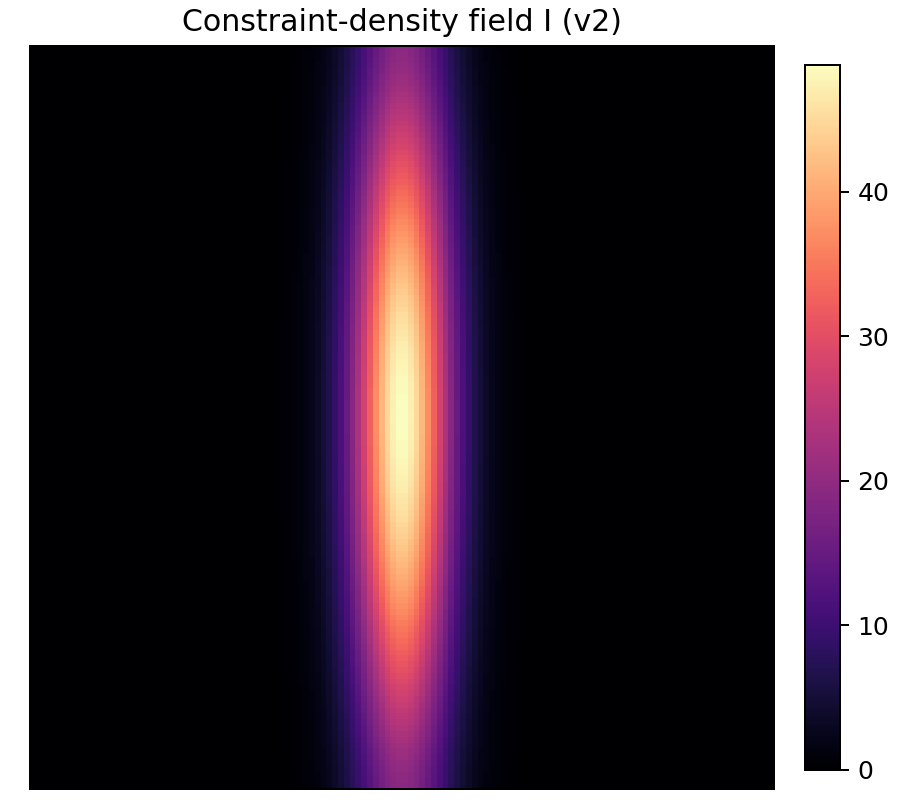
\includegraphics[width=0.70\linewidth]{simulations/minimal_neural_field/outputs/information_density_final_v2.png}
  \caption{最終情報密度 \(\I\)。モルフォゲン場に応じて蓄積し、中央ピークを形成する。}
\end{figure}

\begin{figure}[htbp]
  \centering
  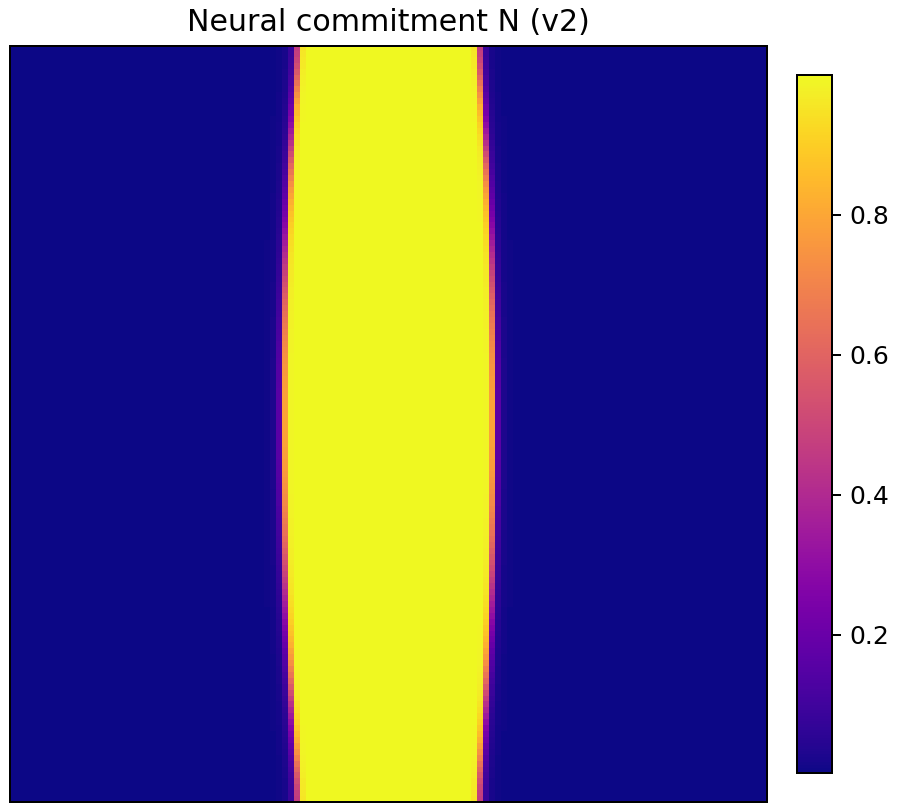
\includegraphics[width=0.70\linewidth]{simulations/minimal_neural_field/outputs/neural_commitment_final_v2.png}
  \caption{最終神経コミットメント \(N\)。情報密度の閾値化により、中央に神経板様領域が形成される。}
\end{figure}

\begin{figure}[htbp]
  \centering
  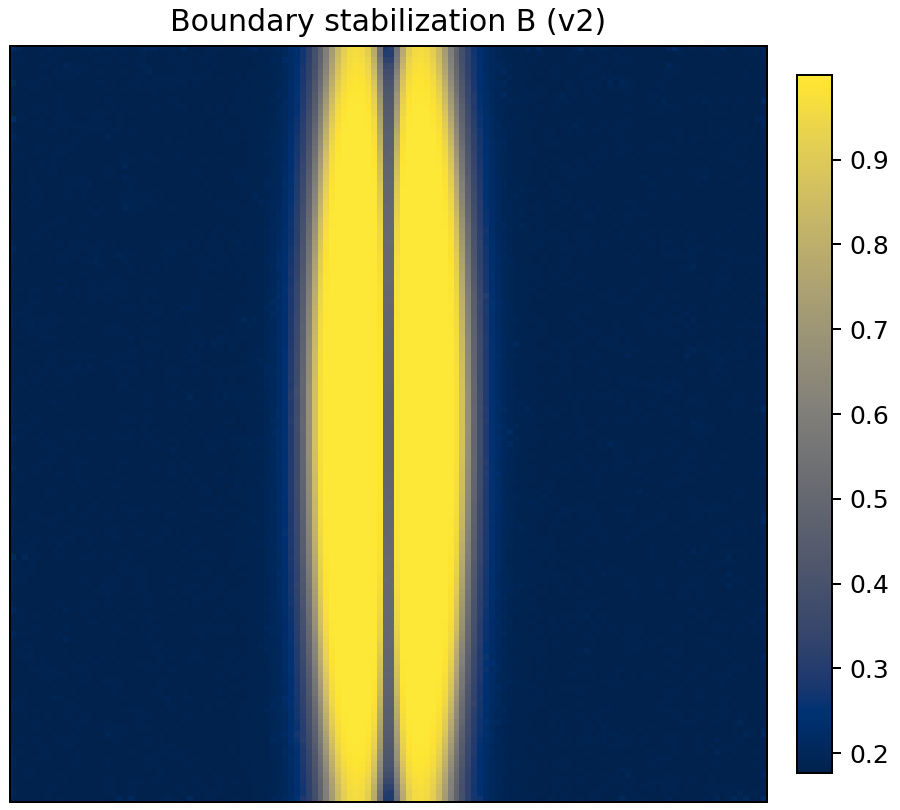
\includegraphics[width=0.70\linewidth]{simulations/minimal_neural_field/outputs/boundary_field_final_v2.png}
  \caption{最終境界安定化場 \(B\)。\(\I\) の勾配構造から導かれ、境界様領域を強調する。}
\end{figure}

\begin{figure}[htbp]
  \centering
  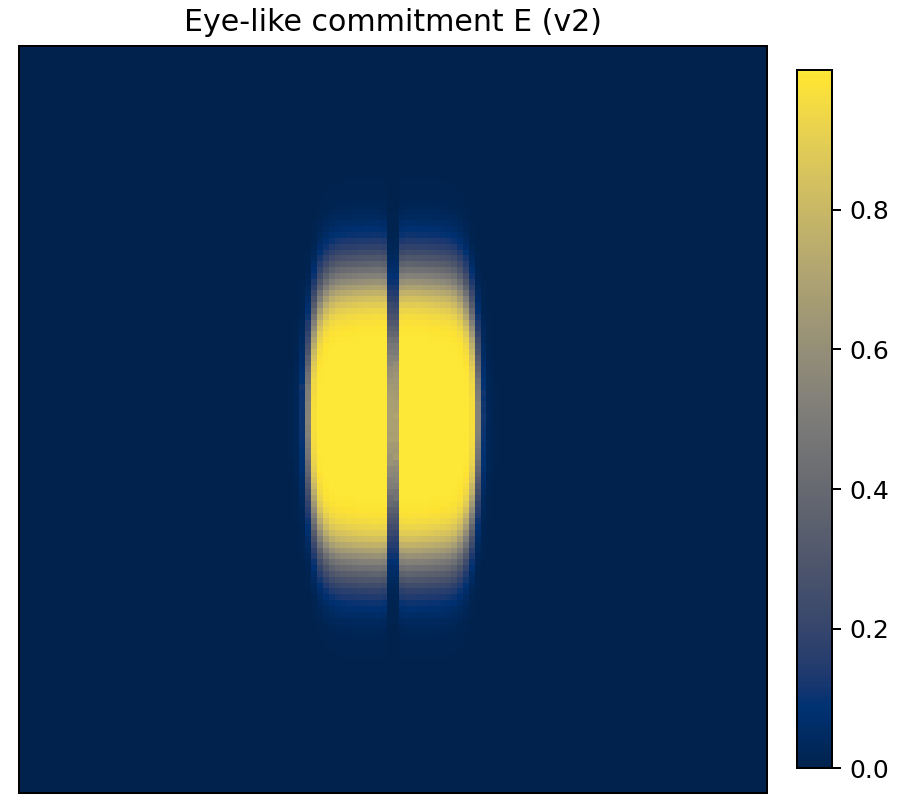
\includegraphics[width=0.70\linewidth]{simulations/minimal_neural_field/outputs/eye_commitment_final_v2.png}
  \caption{最終眼様コミットメント \(E\)。神経コミットメントと境界条件が位置窓内で重なる場所に局所構造が現れる。}
\end{figure}

\begin{figure}[htbp]
  \centering
  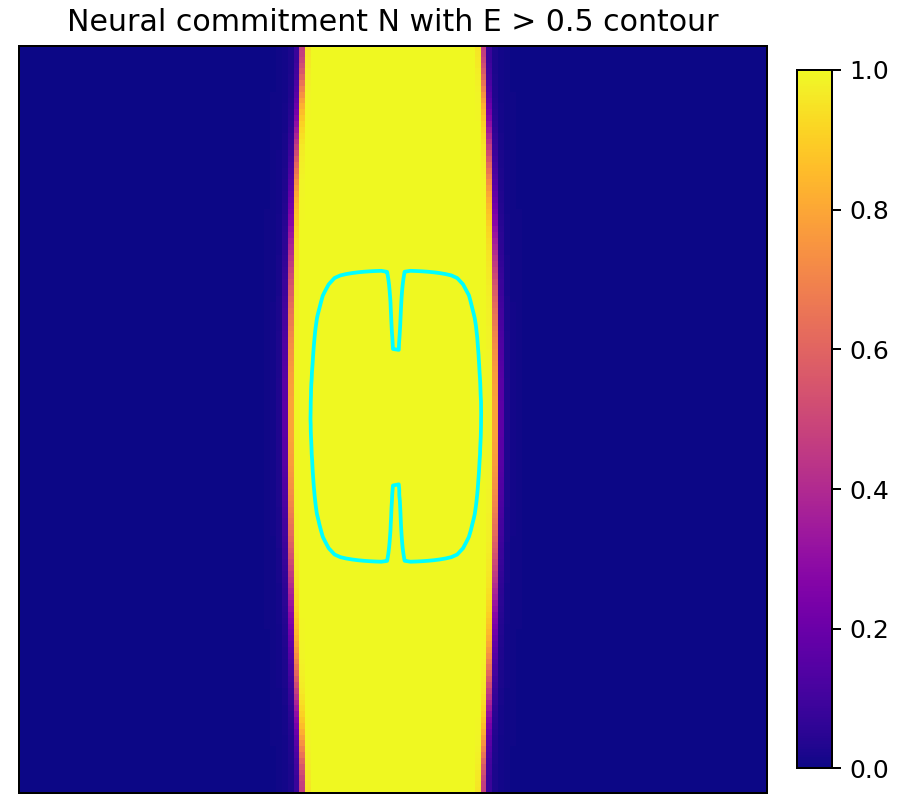
\includegraphics[width=0.70\linewidth]{simulations/minimal_neural_field/outputs/neural_eye_overlay_v2.png}
  \caption{重ね合わせ可視化。背景に \(N\) を示し、閾値化された \(E\) を輪郭として重ねる。}
\end{figure}

\begin{figure}[htbp]
  \centering
  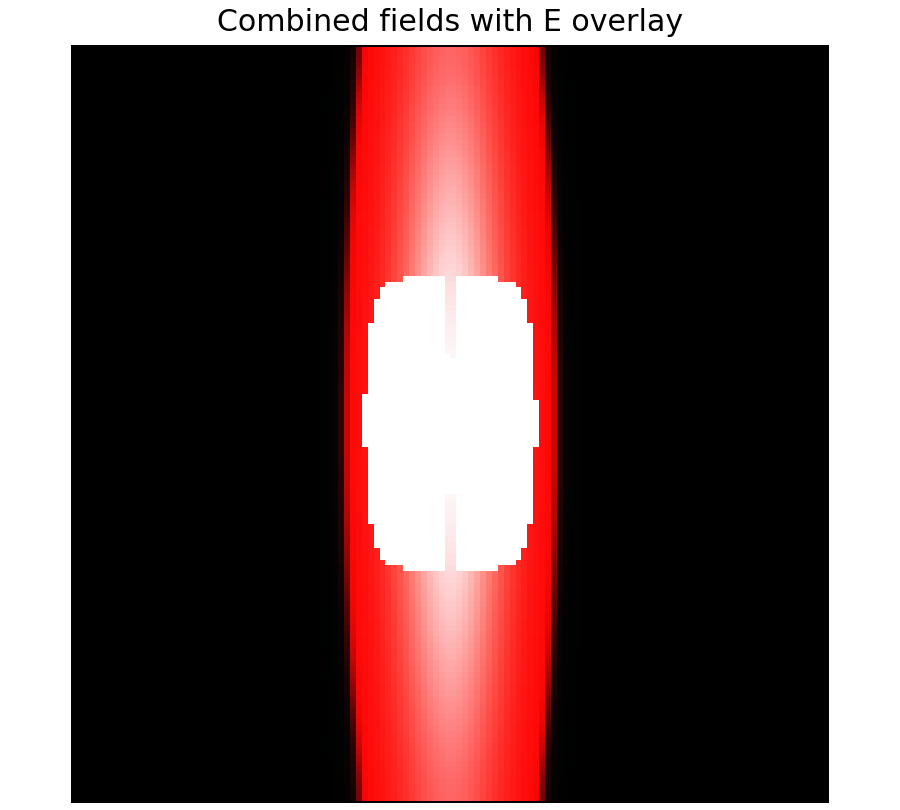
\includegraphics[width=0.70\linewidth]{simulations/minimal_neural_field/outputs/combined_fields_with_eye_v2.png}
  \caption{統合可視化。モルフォゲン場、情報密度、神経コミットメント、眼様コミットメントの最終的な関係を示す。}
\end{figure}

\subsection{時間発展の可視化}

時間発展はアニメーション GIF としても出力されている。
\begin{center}
  \path{simulations/minimal_neural_field/outputs/development_v2_hierarchical.gif}
\end{center}
最小発生モデルの時間発展。単純な動力学的制約のもとで、構造が安定配置として現れる。
このアニメーションは補足資料として提供される。そこでは、モルフォゲン形成、情報密度蓄積、神経板様安定化、境界抽出、二次的な眼様コミットメントの順序が示される。

この順序は
\begin{equation}
  M\rightarrow\I\rightarrow N\rightarrow B\rightarrow E
\end{equation}
という階層的生成経路と一致する。

\subsection{観察のまとめ}

このシミュレーションは、神経板様領域が情報密度の閾値化によって生じること、眼様場が境界構造と位置条件の組み合わせによって生じること、構造が段階的に現れること、最終形が事前に指定されていないことを示す。したがって、結果として得られる構造は、制約されたダイナミクスのもとでの安定解として解釈される。

\subsection{本節の役割}

この結果は、特定の生物現象のモデルではない。本節の役割は、場に基づく動力学系において、最小条件から構造が立ち上がりうることを示す点にある。それは生物学的機構を実証するものではなく、構造的可能性を示すにとどまる。

\clearpage

\section{Discussion}

本節では、本論文で導入した枠組みの射程と限界を整理する。目的は新しい主張を追加することではなく、この枠組みが何を扱い、何を扱わないかを明確にすることである。

本論文は、生物系を情報密度 \(\I\)、情報流 \(\J\)、誘導ポテンシャル \(\PhiI\) によって記述した。この枠組みは、発生、形態形成、生命の持続、知性の成立条件を共通形式で扱うための最小言語である。ただし、個別現象の詳細な再現を目的とするものではない。

本枠組みは、反応拡散系、遺伝子ネットワーク、神経ダイナミクスといった既存モデルを置き換えない。むしろ、それらを密度、流れ、誘導バイアス、安定性という共通構造として再記述するための形式である。

また、この枠組みは完全な平衡や固定閉包への収束を前提としない。流れは継続し、構造は更新され続ける。この意味で、生物系は非閉包的な持続構造として理解される。ただし、この性質は本論文では独立した理論として展開しない。

この解釈は、IFGT において定式化される準閉包構造と整合する。生物系は、閉包が部分的で、動的に維持され、通常の完全閉包状態へ変換されないレジームに留まる。したがって、生物学的ダイナミクスの非閉包性は、この枠組みの限界ではなく、中心的な記述特徴である。

限界も明確である。具体的な生物に対するパラメータ集合 \(\theta\) の導出は扱わない。\(\I\)、\(\J\)、\(\PhiI\) の明示形は系に依存する。数値的予測も与えない。本論文は統一的な記述基盤であり、個別生物系の精密モデルではない。

\section{Conclusion}

本論文では、生物系を情報密度 \(\I\)、情報流 \(\J\)、誘導ポテンシャル \(\PhiI\) によって記述する最小枠組みを示した。この枠組みにより、発生は安定構造への収束として、生命は動的に維持される安定運動として、知性は生命の上に成立する第二のアトラクタとして解釈される。

重要なのは、設計や目的を原始的な説明項として用いなくても、生物学的形態を記述できる点である。本論文はすべての生物学的機構を詳細に再現することを目的としない。生物現象を貫く共通構造を抽出することを目的とする。

本枠組みは、状態、流れ、誘導バイアス、安定性という少数の要素を用いる。これにより、発生、形態形成、生命維持、確率の再定義、知性の成立を一つの記述形式に置くことができる。

残された課題として、具体的な系における \(\theta\) の特定、\(\I\)、\(\J\)、\(\PhiI\) の経験的同定、知性の実装に関する追加モデル化がある。本論文の結果は最終理論ではなく、記述形式である。その有効性は今後の適用と洗練によって評価される。

\end{document}
